\chapter{Realisierung der clientseitigen Implementierung als native App}
\label{cha:native-app}
Dieses Kapitel widmet sich der Implementierung der nativen Applikation. Im Kapitel \ref{cha:architektur} wurde eine grobe Übersicht zu der Umsetzung und der Funktionsweise dieser \ac{App} gegeben, die nun verfeinert wird.
Dabei werden folgend die verwendeten Komponenten und Techniken erläutert und die Zusammenhänge zwischen den Techniken dargestellt.
\section{Allgemeine Funktionsweise einer Android-App}
\label{sec:definition-android}
Grundlegend für die Entwicklung einer Android-App ist das Wissen über die Basis des Systems, auf dem entwickelt wird. 
Bei dem Betriebssystem \ac{Android} handelt es sich um eine Art eines \ac{monolithisch}en Multiuser-\ac{Linux}-Systems. \footcite{Android-Fundamentals}
Dieses Betriebssystem stellt die Hardwaretreiber zur Verfügung und führt die Prozessorganisation, sowie die Benutzer- und Speicherverwaltung durch.
Jede Applikation wird in einem eigenen Prozess gestartet. In diesem Prozess befindet sich eine \ac{Sandbox}, die eine virtuelle Maschine mit der Applikation ausführt. Die Kommunikation aus der Sandbox heraus kann nur über Schnittstellen des Betriebssystems geschehen. Diese Einschränkung sorgt für Sicherheit im System, da ein Prinzip der minimalen Rechte eingehalten wird. Demnach kann eine Applikation nur auf zugewiesene und freigegebene Ressourcen im System zugreifen. Ein weiterer Vorteil dieser internen Architektur liegt in der Robustheit des Systems. Wenn eine Applikation durch Fehler terminiert, wird nur der allokierte Prozess beendet und das Betriebssystem bleibt von diesem Problem unberührt. \footcite{Android-SystemPermissions}
Android-Applikationen werden in der Programmiersprache \ac{Java} geschrieben, mit einem Java-\ac{Compiler} kompiliert und dann von einem Cross-Assembler für die entsprechende \ac{VM} aufbereitet. Das Produkt ist ein ausführbares \ac{.apk}-Paket.\footcite[Seite 17-19]{Android-BeckerPant}
Im Folgenden werden die Android-Komponenten, die für die Umsetzung relevant sind, genauer betrachtet.
\subsection{User Interfaces}
\label{ssec:android-ui}
\textit{User Interfaces} sind die Bildschirmseiten der Android-Applikation. Über diese Seiten wird die Benutzerinteraktion geführt. Das \textit{User Interface} besteht aus zwei Arten von Elementen. Zum einen aus \textit{Views}, die es ermöglichen direkte Interaktionen mit dem Benutzer zu führen. Zu nennen sind dabei \textit{Buttons}, Textfelder und Checkboxen. Als zweites werden \textit{View Groups} verwendet, um \textit{Views} sowie andere \textit{View Groups} anzuordnen.
Das \textit{User Interface Layout} ist durch eine hierarchische Struktur gekennzeichnet. Zum Anlegen einer solchen Struktur gibt es verschiedene Möglichkeiten. Zum einen kann man ein \textit{View}-Objekt anlegen und darauf die Elemente platzieren. Aus Gründen der Performance und der Übersicht ist die Möglichkeit einer \ac{XML}-Datei jedoch zielführender. Aus den Knoten der erstellten Datei werden zur Laufzeit \textit{View}-Objekte erzeugt und angezeigt. Die erzeugten \textit{UIs} werden unter \textit{res/layout} im Android-Betriebssystem hinterlegt. Des Weiteren können Ressourcen in den \textit{UIs} verwendet werden. Unter Ressourcen versteht man Elemente, die zum Verzieren von Oberflächen verwendet werden können. Darunter fallen bespielsweise Grafiken oder \textit{Style-Sheets}, die über den jeweiligen Ressourcen-Schlüssel aufgerufen und verwendet werden.\footcite{Android-UI}
\subsection{Activities}
\label{ssec:android-activities}
\textit{Activities} gehören zu den App-Komponenten, da sie ein grundsätzlicher Bestandteil einer Applikation sind. Es gibt im Normalfall mehrere \textit{Activities} in einer App.\\
Die eigentlichen Aufgaben liegen in der Bereitstellung eines Fensters, das dann auf den Screen, der für die App vom Betriebssystem bereitgestellt wird, gelegt wird. Das Fenster ist im Anschluss für die Annahme von Benutzerinteraktionen bereit. Das Fenster wird mit Hilfe des Aufrufs \textit{SetContentView()} aufgerufen. Zur Benutzerinteraktion werden dann die bereits vorgestellten \textit{View}-Elemente verwendet. Die \textit{Activity} ist folgend für die Verarbeitung und Auswertung der Eingaben verantwortlich.\\
In jeder Applikation muss es eine \textit{MainActivity} geben, die beim Start der Applikation vom Android-Betriebssystem gestartet wird. Zudem muss eine \textit{Activity} im AndroidManifest mit dem Attribut \textit{Launcher} versehen werden, um diese dann als Einstiegspunkt aus dem Menü des Betriebssystems zu setzen. Dabei ist empfehlenswert, dass dieselbe \textit{Activity} sowohl das Main- als auch Launcher-Attribut erhält.\\
Diese Festlegungen müssen im Manifest hinterlegt werden. Das Manifest liegt im Root-Ordner der App und stellt dem Betriebssystem wichtige Informationen der Applikation zur Verfügung. Dieses Manifest wird vor Ausführung der App analysiert und ausgewertet. Darin kann beispielweise festgelegt werden, welche Komponenten oder anderen Applikationen auf entsprechende \textit{Activities} zugreifen dürfen. Wenn eine \textit{Activity} nicht von außerhalb der App erreicht werden soll, sollte kein Intent-Filter gesetzt werden, da demnach der genaue Name der \textit{Activity} zum Start bekannt sein muss. Diese Informationen sind jedoch nur in der gegenwärtigen App vorhanden.\\
Da eine App normalerweise aus mehreren \textit{Activities} besteht, müssen diese \textit{Activities} gestartet werden und untereinander kommunizieren. \textit{Activities} starten sich gegenseitig, weshalb der Aufruf einer \textit{Activity} aus einer anderen erfolgt. Um eine neue \textit{Activity} starten zu können, ist ein Intent von Nöten.
Ein Intent ist ein Nachrichtenobjekt innerhalb von Android, welches zur Kommunikation zwischen App-Komponenten verwendet wird. In diesem Fall zwischen zwei \textit{Activities}. Zur Erstellung benötigt es den Namen der zu startenden Komponente, um eine Verbindung dorthin aufbauen zu können, und eine \textit{Action}, die ausgeführt werden soll. Zudem können Daten übergeben werden, die anschließend als Datenpakete mit dem Aufruf der Komponente mitgegeben werden. Diese Daten sind dann in der gestarteten Komponente aus dem dort vorhandenen Intent auslesbar. Zusätzlich gibt es die Möglichkeit Aktionen vom Betriebssystem ausführen zu lassen. Beispielsweise kann man ein \textit{Intent} mit der Aktion zum Starten des Email-Programms übergeben und die entsprechend im Betriebssystem hinterlegte Applikation zum schreiben von Emails wird geöffnet.\\
Eine \textit{Activity} kann drei Stati in einem \textit{Lifecycle} einnehmen. Zum einen kann die \textit{Activity} im Status \textit{Resumed} - oft auch \textit{Running} genannt - sein und damit momentan im User-Fokus stehen, also im Vordergrund der App sein und die Interaktionen entgegennehmen. Des Weiteren kann eine \textit{Activity} pausieren, wenn eine andere im User-Fokus steht. Dabei ist der \textit{View} der betrachteten \textit{Activity} jedoch immer noch teilweise sichtbar, da der darüberliegende \textit{View} zu Beispiel nicht den gesamten Bildschirm in Anspruch nimmt. Anders verhält es sich, wenn der \textit{View} der betrachteten \textit{Activity} komplett überdeckt ist. Dann befindet sich die \textit{Activity} nämlich im Status \textit{Stopped}. Sowohl im Status \textit{Stopped} als auch im Status \textit{Paused} lebt die \textit{Activity} noch. Das bedeutet, dass das \textit{Activity}-Objekt zusammen mit allen Objekt-Stati und Memberinformationen im Arbeitsspeicher liegt. Der einzige Unterschied dieser beiden Stati liegt darin, dass eine \textit{Activity} im Status \textit{Paused} noch eine Verbindung zum \textit{WindowManager} besitzt, die im Status \textit{Stopped} nicht mehr vorhanden ist. Gemeinsam haben diese beiden Stati jedoch noch, dass sie bei mangelndem Arbeitsspeicher vom Betriebssystem zerstört werden können. 

%ActivityLifecycle-Bild
\begin{figure}[h]
\centering
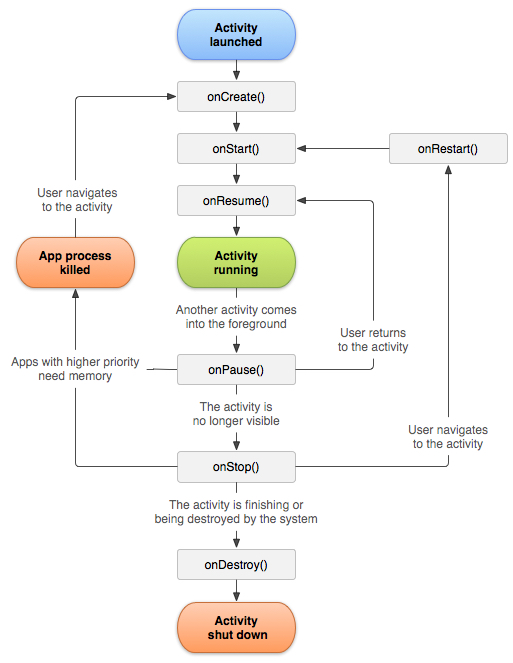
\includegraphics[width=0.8\linewidth]{content/images/Android-ActivityLifecycle}
\caption{Android Activity-Lifecycle}
Quelle: https://developer.android.com/guide/components/activities.html
\label{pic:androidActivityLifecycle}
\end{figure}

Die Ausführung der internen Methoden einer \textit{Activity} ist abhängig von den Eingaben des Benutzers. Dabei durchläuft jede \textit{Activity} ihren \textit{Lifecycle}, der in Abbildung~\ref{pic:androidActivityLifecycle} dargestellt ist. Darin ist zu erkennen, dass zuerst die \textit{OnCreate()}-Methode aufgerufen wird. Darin werden alle essentiellen Initialisierungen gemacht und der \textit{View} aufgerufen. Nachfolgend werden \textit{OnStart()} und \textit{OnResume()} durchlaufen bis die \textit{Activity} den User-Fokus wieder verliert, jedoch der \textit{View} noch sichtbar ist. In dem Moment wird die \textit{OnPause()}-Methode ausgeführt, um Benutzereingaben gegebenenfalls speichern zu können, denn in diesem Zustand ist es in seltenen Fällen möglich, dass der Status - wie oben erklärt - durch das Betriebssystem zerstört wird. Kehrt der Benutzer zurück, wird \textit{OnResume()} wieder aufgerufen, sonst \textit{OnStop()}, um auch dort aufgenommene Daten persitieren zu können. Von dort gibt es zwei verschiedene Rücksprung-Möglichkeiten. Zum einen könnte der Fall eintreten, dass die Daten der \textit{Activity} aus dem Arbeitsspeicher gelöscht wurden, die \textit{Activity} jedoch noch einmal aufgerufen wird. In diesem Fall startet die \textit{Activity} wieder von vorn. Eine weitere Möglichkeit ist die Rückkehr des Benutzers zu der \textit{Activity}. Dabei werden dann die Methoden \textit{OnRestart()} und \textit{OnStart()} aufgerufen.\\
Zusammenfassend lässt sich daraus ableiten, dass die Persistierung von Eingaben in den Methoden \textit{OnPause()}, \textit{OnStop()} und \textit{OnDestroy()} durchgeführt werden sollten, da diese Zustände zerstört werden können. Die weiteren Methoden sollten aus Performancegründen jedoch minimal und agil gehalten werden.
\subsection{Services}
\label{ssec:android-services}
\textit{Services} sind, genauso wie \textit{Activities}, App-Komponenten, die zu den Grundbausteinen einer Android-App gehören. \textit{Services} unterscheiden sich jedoch hinsichtlich ihrer Aufgaben stark von \textit{Activities}. So sind sie dazu da, Aufgaben im Hintergrund zu erledigen. Zudem besitzen sie keinen zugehörigen \textit{View}, sondern werden von anderen App-Komponenten, wie beispielsweise einer \textit{Activity} gestartet. Sie laufen im \textit{Main-Thread} des Prozesses der aufrufenden Komponente. Ein \textit{Service} erstellt keinen eigenen \textit{Thread}, noch einen eigenen Prozess zur Abarbeitung der Aufgaben. Diese Eigenschaft der \textit{Services} muss vom Entwickler bedacht werden. Denn daraus kann man ableiten, dass rechenintensive Aufgaben in einem explizit gestarteten \textit{Thread} arbeiten sollten, um Fehler der Art \textit{Application Not Rsponding} (ANR) zu vermeiden und die Benutzeroberfläche nicht unnötig zu verlangsamen. Ein Vorteil besteht jedoch darin, dass \textit{Services} Aufgaben auch dann noch ausführen können, wenn die App, zu der sie gehören, geschlossen wurde. So können noch nicht abgeschlossene \textit{Up-} oder \textit{Downloads} noch beendet werden oder das Abspielen von Musik bei ausgeschaltetem Bildschirm fortgeführt werden.\\
Bei Android wird grundsätzlich zwischen zewi Arten von \textit{Services} unterschieden. Zum einen gibt es \textit{Started-Services}, die durch eine App-Komponente mit dem Befehl \textit{StartService()} gestartet werden. Grundsätzlich ist dieser Aufruf uneingeschränkt von allen App-Komponenten möglich, soweit die Einstellungen im Android-Manifest diese zulassen. Weiterhin laufen \textit{Started-Services} im Hintergrund der App weiter, auch wenn die Komponente, die den \textit{Service} gestartet hat, zerstört oder beendet wurde. Deshalb führt diese Art des \textit{Services} im Normalfall eine Aufgabe aus und stoppt sich anschließend nach der Fertigstellung selbstständig. Auf der anderen Seite gibt es \textit{Bound-Services}, die durch einen Aufruf von \textit{BindServcice()} einer anderen App-Komponente gestartet werden. In diesem Schritt verbinden sich die Komponente und der \textit{Service} über eine Art \textit{Client-Server Interface}, das zur Kommunikation bereitgestellt wird. Dieses \textit{Interface} ist vom Typ \textit{IBind} und sorgt für den Austausch von \textit{Request} und \textit{Results}. Des Weiteren verläuft eine mögliche Interprozess-Kommunikation zwischen Komponente und \textit{Service} über dieses \textit{Interface}. Die größte Besonderheit eines \textit{Bound-Services} besteht darin, dass der \textit{Service} nur so lange besteht, wie mindestens eine Komponente an diesen gebunden ist. Natürlich ist es möglich, dass sich mehrere Komponenten gleichzeitig an diesen \textit{Service} binden können. Löst sich jedoch die letzte Komponente wieder, wird der \textit{Service} zerstört. Natürlich gibt es Mischformen dieser beiden \textit{Service}-Arten, die abhängig von der zu leistenden Aufgabe gewählt werden sollten. 

%ServiceLifecycle-Bild
\begin{figure}[h]
\centering
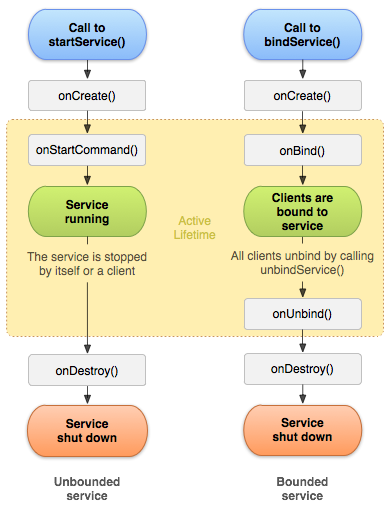
\includegraphics[width=0.8\linewidth]{content/images/Android-ServiceLifecycle}
\caption{Android Service-Lifecycle}
Quelle: https://developer.android.com/guide/components/services.html
\label{pic:androidServiceLifecycle}
\end{figure}

Zum Erstellen eines \textit{Services} muss von der Klasse \textit{Service}, oder davon abgeleitete Klassen, geerbt werden. Danach müssen die vorgegebenen Methoden überschrieben werden, denn \textit{Services} besitzen, genauso wie \textit{Activities}, einen Lebenszyklus. Dabei muss jedoch wieder zwischen den beiden Arten von \textit{Services} unterschieden werden.\\
\textit{Started-Services} werden die Methode \textit{OnCreate()} nach dem Start durch eine Komponente ausführen, wenn der \textit{Service} noch nicht läuft. Darin sollten dann die Initialisierungen und einmaligen Aufgaben zum Start des \textit{Services} durchgeführt werden. \textit{OnStartCommand()} wird immer dann aufgerufen, wenn der \textit{Service} wieder von einer Komponente aufgerufen wird. Dann befindet er sich im Zustand \textit{Running} und führt die ihm zugewiesenen Aufgaben durch. Wenn der \textit{Service} zerstört wird, sei es durch Speichermangel des \textit{Devices} oder das Beenden durch eine Komponente oder den \textit{Service} selbst, wird \textit{OnDestroy()} ausgeführt, um abschließende Aufgaben durchzuführen. Dazu zählen beispielsweise das Beenden von Datenbankverbindungen oder \textit{Threads}.\\
\textit{Bound-Services} werden, wie oben genannt, über \textit{BindService()} von einer Komponente gestartet und führen dann, genauso wie die \textit{Started-Services}, die \textit{OnCreate()}-Methode zum Initialisieren aus. Gefolgt vom aktiven Status, in dem anfangs \textit{OnBind()} aufgerufen wird und die von den Komponenten verlangten Aufgaben ausgeführt werden. Anschließend lösen sich die Komponenten wieder vom \textit{Service}. Haben sich alle Komponenten gelöst, wird auch beim \textit{Bound-Service} \textit{OnDestroy()} ausgeführt.
\subsection{Prozesse und Threads}
\label{ssec:android-prozesse-threads}
Sobald eine Applikation gestartet wird, und keine Komponenten daraus bereits laufen, wird vom Android-Betriebssystem ein neuer Prozess mit einem dazugehörigen \textit{Main-Thread} erzeugt. Standardmäßig werden alle Operationen dieser App in diesem Prozess und diesem \textit{Thread} ausgeführt. Laufen Teile einer Applikation jedoch noch im Hintergrund, wie es bei Services möglich ist (siehe \ref{ssec:android-services}), und die App wird vom Benutzer erneut gestartet, so wird diese Komponente in dem noch bestehenden Prozess und \textit{Thread} eingepflegt.\\
Es gibt jedoch auch die Möglichkeit verschiedene App-Komponenten auf mehrere Prozesse zu verteilen. Dazu genügt ein Eintrag im Android-Manifest. Dadurch ist es dann auch möglich Komponenten verschiedener Applikationen in einem Prozess laufen zu lassen. Voraussetzung dafür ist, dass diese beiden Applikationen mit demselben Zertifikat generiert wurden und dieselbe Linux \textit{\ac{user ID}} besitzen.\\
Prozesse können aber auch durch das Betriebssystem zerstört werden, wenn die Geräte-Ressourcen sich zum Beispiel dem Ende neigen und neue freigegeben werden müssen. Hierzu gliedert Android die Prozesse in eine Hierarchie ein und beendet die Prozesse, die zum Beispiel vom Benutzer seit längerer Zeit nicht mehr verwendet wurden oder keinen direkten Kontakt zur aktuellen Anzeige besitzen.\\
Der angesprochene \textit{Main-} oder auch \textit{\ac{UI-Thread}} beim Starten einer App, ist der Hauptakteur für die Kommunikation mit dem Betriebssystem. So werden alle Aufrufe an die Komponenten des \textit{Android UI toolkits} über diesen \textit{Thread} abgewickelt. Demnach müssen über diesen \textit{Thread} alle \textit{Callback}-Methoden von Systemeigenschaften, wie \textit{OnClick()}, darin bearbeitet werden. Daraus ergibt sich, dass aufwendige Aufgaben, die zum Beispiel Netzwerkverbindungen verwenden, in andere \textit{Threads} verlagert werden sollten, um dem Benutzer eine Oberfläche ohne lästige Wartezeiten zu ermöglichen. Einzige Einschränkung dabei ist, dass niemals von einem anderen \textit{Thread} als dem \textit{UI-Thread} auf \textit{\ac{Android UI toolkits}} zugegriffen werden darf. Diese Limitierung muss bei der Implementierung beachtet werden.\\
Zum Umgehen dieser Problematik können asynchrone \textit{\ac{Tasks}} verwendet werden, die Aufgaben außerhalb des \textit{UI-Threads} ausführen. Auf das Ergebnis dieser Ausführungen kann dann wieder zugegriffen werden. Diese Umsetzung bietet einen leichteren Umgang mit \textit{Multithreading} für den Entwickler und genießt deshalb immer größere Beliebtheit.
\subsection{SQLite}
\label{ssec:android-sqlite}
SQLite ist eine in sich geschlossene und serverlose \ac{SQL}-Datenbank. Sie besteht aus einer \textit{In-Process}-Bibliothek, die es ermöglicht eine Datenbank ohne eigenen Server-Prozess zu betreiben. Dabei liegt die Datenbank mitsamt aller Tabellen, \textit{Views} und \textit{\ac{Trigger}} in einer einzigen Datei vor. Diese Datei ist zudem so konzipiert, dass sie plattformübergreifend zwischen 32- und 64-Bit-Systemen kopiert werden kann. Weitere Vorteile von SQLite liegen in der sehr sparsamen Speicherung der Daten und der, durch die gemeinfreie Lizenz, große Unterstützung durch Drittanbieter-Programmen. So gibt es für alle gängigen mobilen Systeme eine meist schon integrierte Unterstützung von SQLite-Datenbanken. Android unterstützt diese Datenbankart als präferierte Datenhaltung.
\section{Was ist Xamarin Platform?}
\label{sec:defintion-xamarin}
Xamarin Platform ist ein Produkt der Firma Xamarin, die ihren Sitz in San Francisco hat. Diese Firma entwickelt Software für die Erstellung von nativen Apps auf Basis des \textit{Open Source}-Projekts \ac{Mono}. Mono seinerseits hat mehrere Vorteile:
\begin{itemize}
\item \textbf{Popularität}\\Es kann auf die Erfahrung von Millionen C\# -Entwicklern zurückgegriffen werden.
\item \textbf{Höhere Programmiersprache} \\Es können die Vorteile von höheren Programmiersprachen verwendet werden. Zu nennen sind dabei besonders \textit{Threading}, automatische Speicherverwaltung und \textit{\ac{Reflection}}.
\item \textbf{Klassenbibliotheken}\\Die Verwendung von bestehenden Klassenbibliotheken erleichtern das Umsetzen komplexer Aufgaben.
\item \textbf{\textit{Cross-Platform}}\\Die fertiggestellte Software kann auf fast allen Systemen verwendet werden.
\end{itemize}
Damit können plattfomunabhängige Programme in C\# programmiert werden. Beliebtheit erlangte Mono mit dem Wunsch von Entwicklern Apps auf verschiedenen mobilen Betriebssystemen bereitstellen zu können und dabei Änderungen und die Entwicklung größtmöglich zu vereinen. Genau diese Wünsche werden mit \textit{Xamarin Platform} erfüllt. Vorher war es immer nötig drei Applikationen für die verbreitetsten mobilen Betriebssysteme zu entwickeln. Dies bedeutete, dass die \textit{Guidlines} der jeweiligen Systeme iOS, Android und Windows Phone analysiert und in den jeweiligen Programmiersprachen umgesetzt werden mussten.
\subsection{Multiplattform-Unterstützung}
\label{ssec:xamarin-multiplattform}

%Xamarin-Platform-Bild
\begin{figure}[h]
\centering
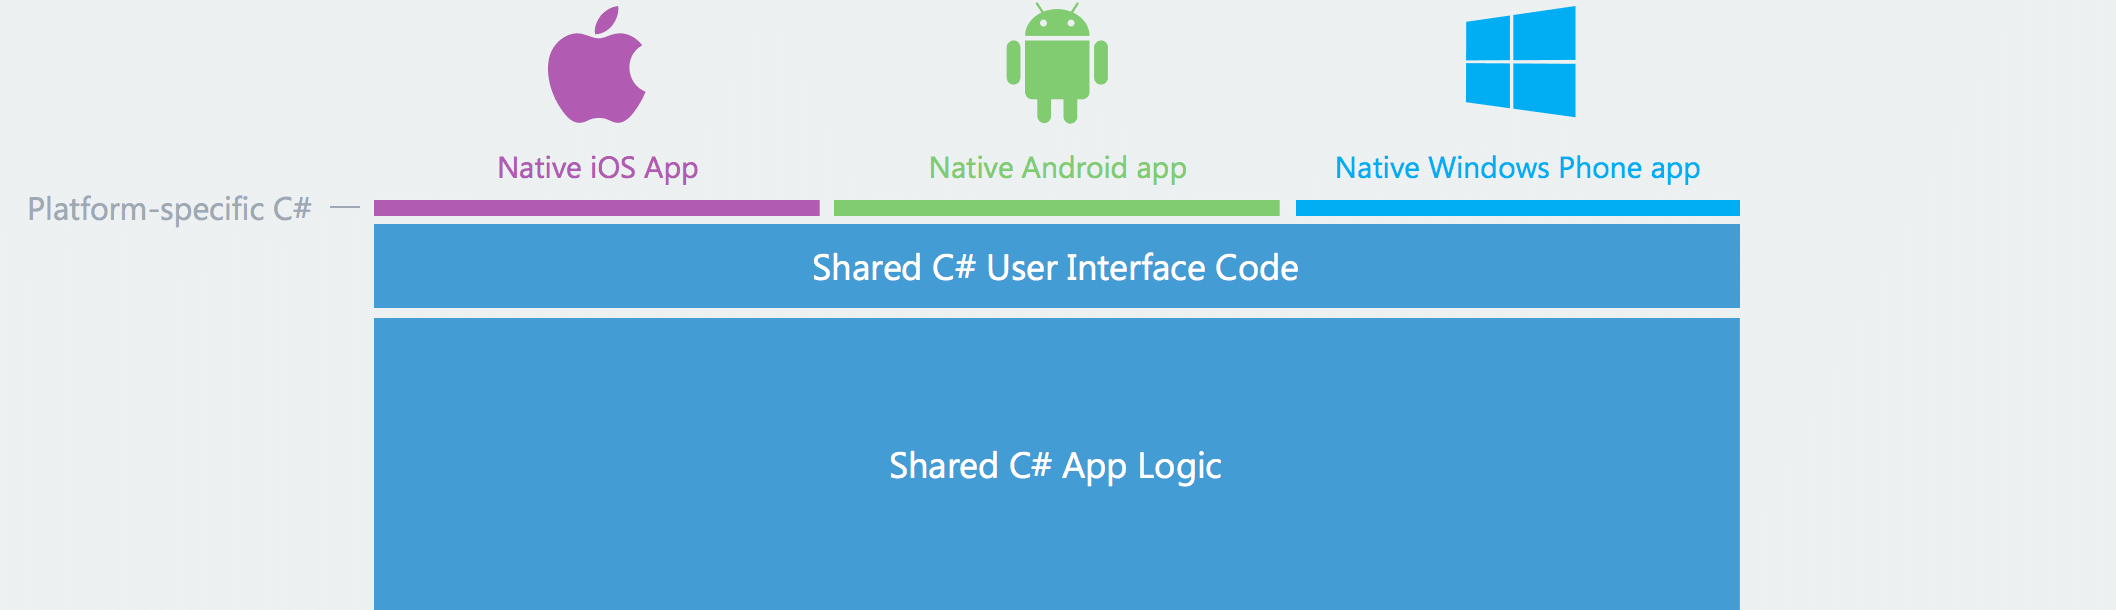
\includegraphics[width=\linewidth]{content/images/Xamarin-Platform}
\caption{Xamarin Platform}
Quelle: http://xamarin.com/platform
\label{pic:xamarinPlatform}
\end{figure}

Durch Xamarin Platform ist es möglich alle Funktionalitäten der gewünschten Betriebssysteme in vollem Umfang zu verwenden. Diese Tatsache liegt daran, dass erstellte Projekte in die nativen Sprachen des Systems überführt und dann normal kompiliert werden. Durch die Nutzung der Standard-Steuerelemente eines jeden Betriebssystems sorgt dafür, dass die Benutzer keinen Unterschied zu einer App erkennen können, die ausschließlich für ein Betriebssystem entwickelt wurde. Auch plattformspezifische Funktionen können verwendet werden. Zudem werden alle Vorteile der Programmiersprache C\# ausgenutzt.\footcite{Xamarin-Platform} So ist der Umgang mit asynchronen Funktionen in dieser Sprache zum heutigen Stand am besten gelöst. Des Weiteren können \textit{Shared Projects} zur Entwicklung verwendet werden, sowie \ac{PCL}s und \textit{\ac{NuGet}}-Pakete eingebunden werden, um den Funktionsumfang schnell und einfach erweitern zu können.\footcite{Xamarin-Multiplatform}
\subsection{Besonderheiten der Android-Umsetzung}
\label{ssec:xamarin-android}
Bei der Entwicklung einer Android-App mit Hilfe von Xamarin Platform vereint man die Vorteile zweier Systeme. Zum einen hat man den Vorteil der freien und starken Entwicklungsumgebung Visual Studio in Kombination mit C\#, zum anderen kann man alle Besonderheiten der Android-Entwicklung einbeziehen und verwenden.\\
So muss man am Anfang der Entwicklung auswählen, welche Android-\ac{API} als Minimalvoraussetzung verwendet werden soll und welche Version vorrangig unterstützt werden soll. Zweifellos ist es möglich die von dem \textit{Device} verwendete Android-Version abzufragen und dementsprechend die Funktionalität der App anzupassen.
Zudem können \textit{Java-Packages} eingebunden und verwendet werden, um bekannte Funktionen auch in C\# verwenden zu können.\\
Eine sehr große Unterstützung ist das automatische Führen des Android-Manifestes. Dabei werden zwar nur rudimentäre Einstellungen aus der Entwicklung übernommen, aber auch diese Unterstützung ist für Neulinge auf dem Gebiet der Android-Entwicklung eine gute Beihilfe.
\subsection{Android Emulator}
\label{ssec:xamarin-emulator}
Zum Testen der Android-App konnte ein Emulator verwendet werden, der in dem Xamarin-Plugin für Visual Studio bereitgestellt wurde. Damit konnten dann verschiedene Szenarien, wie Verbindungsverlust oder Speicherknappheit, nachgestellt werden. Für die App wurde das Android-API-Level 19 als Minimal- und \textit{Target}-Anforderung gewählt. Dies steht für Android 4.4 mit dem Namen Kitkat. Damit sollte eine große Abdeckung von Android-Geräten bewerkstelligt werden.\footcite{Xamarin-API}
\section{Eigene Umsetzung}
\label{sec:nat-umsetzung}
Im folgenden wird auf die Umsetzung der nativen Android-Applikation mit Hilfe von Xamarin Platform eingegangen. Anfangs wurde beim Anlegen des Projektes das Android-API-Level, wie oben beschrieben, auf 19 gesetzt und die Entwicklung darauf abgestimmt.

\subsection{Anlegen der Layouts}
\label{ssec:nat-layouts}
Der Aufbau der Layout-Seiten ist auf Grund einer vorher abgestimmten \textit{User-Guideline} vorgenommen worden. So entsteht eine Übersichtsseite, auf der der Benutzer entscheiden kann, ob er sich einloggt oder registriert.
Zu Beginn des Anlegens dieses \textit{Main-Layouts} wurde ein \textit{ViewGroup} des Typs \textit{LinearLayout} gewählt, um die \textit{Widget}-Elemente darauf anzuordnen. Hinzugefügt wurden demnach zwei \textit{Buttons} für die genannten Funktionen, ein Text für die Überschrift, sowie eine \textit{ImageView}, die für die Anzeige der Konnektivität zum Server verwendet wird.\\
Bei einem \textit{Click} auf den Registrieren-\textit{Button} erscheint ein Dialog im Vordergrund, der den Benutzer dazu auffordert die benötigten Daten zur Registrierung einzugeben. Die Oberfläche orientiert sich demnach an einem \textit{RelativeLayout}, um die \textit{Widgets} darauf anzulegen. Zur Vereinfachung der Validierung wird für das Eingabefeld der Email-Adresse ein \textit{EditText-Widget} mit dem \textit{InputType} \textit{textEmailAddress} verwendet. Somit wird die Benutzereingabe in diesem Feld vom Betriebssystem auf die Eigenschaften einer Email-Adresse überprüft. Intern wird dazu eine \textit{Regular Expression} zur Validierung verwendet und die Überprüfung kann vernachlässigt werden.\\
Zur Weitergabe der Eingabedaten muss eine von \textit{EventArgs} erbende Klasse erstellt werden, die alle Daten zur Registrierung hält. Die Eingabe des Passwortes und der Wiederholung des Passwortes wird in einem speziellen Passwort-Feld entgegengenommen. Dadurch wird die für Passwörter bekannte Eingabe vom Betriebssystem verwendet. Die Buchstaben werden als Punkte dargestellt und sind somit nicht so leicht für Dritte bei der Eingabe einsehbar.\\
Zur Aufnahme der Daten Geschlecht, Job und Beruf gibt es vorher definierte Daten für die Eingabe auf dem Server. Dabei hat sich anfangs die Schwierigkeit ergeben, dass die \textit{Spinner}, die scrollbaren Auswahlfelder, mit den festgelegten Daten besetzt und dann in dem entsprechenden Datentypen wieder ausgelesen werden müssen. Die Belegung der \textit{Spinner} erfolgt über einen typisierten \textit{ArrayAdapter}, der die Werte des übergebenen \textit{Enums} ausgibt. Das Einlesen des ausgewählten Wertes wird über jeweils eine ausgelagerte Funktion geregelt, die die Auswahl, die als \textit{String} erhalten wird, in den jeweiligen Typ parst. Anhand der erhaltenen \textit{ServerException} wird dann ausgegeben, welche Eingabe für die Registrierung falsch eingegeben wurde. Dies ist auch einer der Gründe, weshalb die Registrierung nur im Online-Modus der App unterstützt wird. Zudem muss der Server überprüfen, ob der Benutzername verwendet werden kann. Nach der erfolgreichen Registrierung verschwindet der Dialog wieder und die Konnektivitätsanzeige der Startseite wird mit dem aktuellen Status belegt. Dies geschieht nicht beim Statuswechsel, da dies mit der Architektur der Online-Status-Abfrage in Verbindung steht. Diese wird in einem eigenen \textit{Thread} durchgeführt und dieser kann keine Änderungen an der Oberfläche vornehmen. Eine Verbesserungsmöglichkeit wäre deshalb ein Aufruf in dem Abfrage-\textit{Thread}, der dann auf dem \textit{UI-Thread} ausgeführt wird. Dann würde die Anzeige immer direkt beim Statuswechsel aktualisiert werden.\\
Beim Login besteht das Dialogfenster aus den beiden Eingabefeldern für Benutzername und Passwort, sowie einem Login-Knopf. Beim Betätigen des Knopfes wird die Kombination \textit{Username} und Passwort beim \textit{OnOffServiceLocal} abgefragt. Bei einer ungültigen Eingabe wird ein Hinweis an dem Feld des Passwortes angezeigt, der angibt, dass die Login-Daten falsch sind und eine erneute Eingabe ist erforderlich. Aus sicherheitstechnischen Gründen wird nicht angegeben, ob der Benutzername schon nicht in der Datenbank vorhanden ist, oder, ob nur die Kombination fehlerhaft ist. Nach einer validen Eingabe verschwindet der Login-Dialog wieder und die Startseite ist für drei Sekunden sichtbar, um einen Blick auf die Konnektivitätsanzeige werfen zu können. Danach folgt eine Weiterleitung zu den Trainingsplänen des nun eingeloggten Benutzers.\\
Die Darstellung der Trainingspläne und der zugehörigen Übungen auf einer folgenden Seite sind technologisch gesehen gleich. Einzig die Beziehung der zu ladenden Daten und die übergebenen Werte ändern sich. Als herausfordernd hat sich das Belegen der \textit{ListView} zur Anzeige der tabellarischen Daten und die Weitergabe der \textit{ScheduleId} und der \textit{UserId} herausgestellt. Die \textit{ScheduleId} und die \textit{UserId} werden benötigt, um die Übungen zu einem Trainingsplan herauszufinden. Aber zuerst wurde die Erstellung der \textit{ListView} gelöst. Dafür sind ein \textit{ScheduleListViewAdapter} und ein \textit{ScheduleView} von Nöten. Der \textit{ListViewAdapter} erweitert die Klasse \textit{BaseAdapter} und gibt bei einem Klick die Position des Elements im \textit{Array} der Trainingspläne zurück. Das unsichtbare Feld \textit{txtScheduleViewID} im \textit{ScheduleView} ist notwendig, um dieses bei einem Klick auslesen zu können und dann an die folgende Übersichtsseite der Übungen übergeben zu können.\\
Zur Übergabe der \textit{UserId} und der \textit{ScheduleId} an die \textit{ExerciseActivity} wurde zuerst vergeblich versucht diese im Aufruf der \textit{ExerciseActivity} mit zu übergeben. Diese Möglichkeit hat sich im Nachhinein als Irrtum herausgestellt und eine weitere Einarbeitung in die vorherig erläuterten \textit{Intents} (siehe Kapitel \ref{ssec:android-activities}) durchgeführt. Danach setzte sich die Umsetzung dahingehend weiter, dass die Funktion \textit{PutExtra()} des \textit{Intents} dazu genutzt wurde, um die Daten zu übertragen. In der \textit{ExerciseActivity} werden diese dann wieder ausgelesen und weiterverwendet. Beide Werte sind essentiell, um die Übungen des angemeldeten Benutzers zu seinem ausgewählten Trainingsplan zu erhalten.\\
\lstinputlisting[caption=Übertragen von Daten zwischen Activities, label=lst:ExerciseActivity, style=sharpc]{content/listings/ExerciseActivity.cs}
Bei der Übergabe der Daten an die \textit{PracticeActivity} wird zudem noch die \textit{ExerciseId} übertragen, um alle nötigen Fremdschlüssel für das Anlegen des Trainings zu besitzen.\\
Eine Anmerkung zu der Übergabe der \textit{UserId}: Diese muss über die \textit{Activities} übertragen werden und kann nicht einfach aus der aktuellen \textit{UserSession} des Benutzers gelesen werden, da man davon ausgehen muss, dass sich der Benutzer auch offline hätte einloggen können. Demnach hat man im Online-Modus zwei Möglichkeiten die Id des \textit{Users} zu erhalten, im Offline-Modus hingegen ist dies die einzige Lösung.\\
\lstinputlisting[caption=Auslesen von Daten zwischen Activities, label=lst:PracticeActivity, style=sharpc]{content/listings/PracticeActivity.cs}
Wie im Codebeispiel ersichtlich kann man die übergebenen Informationen zwischen \textit{Activities} aus dem \textit{Intent} auslesen. Zudem kann man erkennen, dass man dank Xamarin das Parsen einer \textit{Integer}-Zahl über eine \textit{Java}-Funktion durchführen kann.\\
Im folgenden Kapitel wird dann auf den noch unbekannten Aufruf des \textit{ooService}-Objekts eingegangen.
\subsection{OnOffService}
\label{ssec:nat-onoffservice}
Dieser \textit{OnOffService} ist die Schicht zum verteilen der An- und Abfragen, abhängig von dem Verbindungsstatus. Demnach werden immer Methoden dieser Klasse von den \textit{Activities} aufgerufen, wenn Daten abgerufen oder abgelegt werden sollen. Dann wird in der Methode eine Unterscheidung gemacht, ob das \textit{Device} gerade online oder offline ist und dementsprechend die Interaktion mit der lokalen Datenbank (siehe Kapitel \ref{ssec:nat-db}) oder dem Server durchgeführt. Zudem wird dabei immer die Konvertierung verschiedener Typen durchgeführt, die durch die Architektur nötig wurden.
\lstinputlisting[caption=Login über den \textit{OnOffService}, label=lst:OnOffService, style=sharpc]{content/listings/OnOffService.cs}
In diesem Codebeispiel kann man die Umsetzung dieser Aufgabe an Hand des Logins erkennen. Zum Aufbau der lokalen Datenhaltung wird in diesem Schritt schon der User, der sich gerade einloggt, mit der \textit{UserId} gespeichert. Die \textit{Exceptions} werden bewusst nicht alle in diesem Schritt behandelt, um die aufrufende \textit{Activity} mit der originalen Fehlermeldung des Servers versorgen zu können und den Fehler dann in der Oberfläche darstellen zu können.\\
Alle Methoden der Klasse \textit{OnOffService} sind asynchron. Das liegt zum einen an den asynchronen Aufrufen, die an den Server gestellt werden. Es würde die Performancevorteile verspielen, wenn man diese asynchronen Methoden dann beim Serverabruf synchron verwenden würde. Auf der anderen Seite sollten dadurch die Performancevorteile der Asynchronität in diese App übernommen werden. Auch wenn dabei noch Verbesserungen in der App vorgenommen werden können, um die Ressourcen des Gerätes optimal auszunutzen. Unter Verwendung eines eigenen \textit{Threads} zum Abarbeiten der Server-Anfragen könnten weitere Leistungssteigerungen erreicht werden. Dabei wurde dann aber der Aufwand und die Probleme der \textit{Thread}-Synchronisierung als ein für diese Arbeit zu großer Aufwand geschätzt. Besonders, da die Server-Methoden großteils Rückgabewerte liefern, die für die Weiterverarbeitung essentiell sind. Möglich wäre diese Optimierung mit einem startenden \textit{Thread} in den Server-Aufrufen, die dann neben dem \textit{UI-Thread} laufen und bei Fertigstellung die benötigten Daten wieder in den startenden \textit{Thread} übertragen. Damit würde man eventuelle Ladezeiten der Oberfläche minimieren oder sogar vollständig verhindern.

\subsection{Lokale Datenbank}
\label{ssec:nat-db}
Technologisch wird eine SQLite-Datenbank aus den bereits in Kapitel \ref{ssec:android-sqlite} erläuterten Vorteilen genutzt.\\
Die lokale Datenbank dieser App wird für die Umsetzung des \textit{Caches} (siehe Kapitel \ref{ssec:nat-cache}) benötigt. Darin werden die lokalen Daten gespeichert und mit dem Server abgeglichen.
Die Erstellung der Datenbank findet beim Start des \textit{OnOffServices} statt. Ist die Datenbank schon vorhanden, wird keine weitere Aktion ausgeführt. Zur Verbesserung der Leistung wird die Erstellung in einem separaten Thread durchgeführt, da kein Rückgabewert erwartet wird. Die zur Erstellung der Server-Datenbank verwendeten Models konnten in diesem Zusammenhang nicht verwendet werden, da die Annotation der OR-Mapper nicht äquivalent sind. Des Weiteren ist es nicht möglich Fremdschlüssel in SQLite zu deklarieren. Diese wurden nun programmatisch oder über Beziehungstabellen gepflegt. Daraus ergibt sich eine Verbesserungsmöglichkeit für eine neue Version der Applikation. Als hilfreich könnte sich dabei eine \textit{SQLite-Extension} herausstellen, die der Datenbank dann einen größeren Funktionsumfang schenken und die Anzahl der direkten SQL-Befehle minimieren würde. Diese wurde testweise eingepflegt, funktionierte aber nicht erwartungsgemäß.\\
\lstinputlisting[caption=\textit{UserModel} für die lokale Datenbank, label=lst:DBModels, style=sharpc]{content/listings/DBModels.cs}
Der lokale \textit{User} besitzt eine lokale Id als \textit{PrimaryKey} zur Identifizierung. Geplant war im Vorfeld jedoch eine Kombination aus \textit{wasOffline} \textit{LocalId}. Da SQLite jedoch keinen \textit{PrimaryKey} aus zwei Attributen unterstützt, musste diese Überlegung verworfen werden. Die gespeicherte \textit{UserId} ist der Guid vom Server, der als \textit{Session}-Ersatz gehalten wird. Die anderen benötigten Tabellen werden nach diesem Muster auch erstellt.\\
Die Interaktion mit der lokalen Datenbank wird synchron durchgeführt, da die asynchrone Schnittstelle nicht alle benötigten Methoden zur Verfügung stellt. Beim Zugriff zur Datenbank wird auf eine Mischung aus direkten SQL-Befehlen und der Nutzung von SQLite-Methoden zurückgegriffen. Einfache Such- oder Einfüge-Operationen werden vom \textit{Framework} bereitgestellt, wohingegen Abfragen über die erstellten Beziehungstabellen selbst umgesetzt wurden.
\subsection{Lokaler ManagementService}
\label{ssec:nat-ManagementServiceLocal}
Die Verbindung zum Server geschieht über das bereitgestellte \textit{Package} fIT.WebApi.Client.Portable. Alle benötigten Funktionen werden darin bereitgestellt. Darüber wird dann die Kommunikation über REST mit dem Server abgewickelt.\\
In der App wird der \textit{ManagementService} zum Verbindungsaufbau verwendet. Da ein internes Routing über den \textit{OnOffService} durchgeführt wird, die Verbindung zur lokalen Datenbank von der \textit{LocalDB} gemacht wird, gibt es zur Verbindung zum Server den \textit{ManagementLocalService}. Dieser \textit{Service} arbeitet mit dem Server direkt zusammen und ist ausschließlich für das Abrufen von Daten vom Server verantwortlich. Rückgabewerte werden meist einfach weitergereicht.\\
Zur Veranschaulichung ein kleiner Ausschnitt aus dem Online-Login, der veranschaulicht, wie die Kommunikation aufgebaut wird.
\lstinputlisting[caption=Login am Server, label=lst:ManagementServiceLocal, style=sharpc]{content/listings/ManagementServiceLocal.cs}
\subsection{Verbindungsprüfung zum Server}
\label{ssec:nat-konnektivität}
Die Verbindungsprüfung zum Server geschieht im \textit{OnOffService}. Dafür wird eine unendliche Schleife in einem eigenen \textit{Thread} gestartet, um in einem festen Intervall (alle 10 Sekunden) einen \textit{Ping} zum Server zu schicken und damit die Erreichbarkeit des Servers zu überprüfen. Diese Methode wird vom \textit{ManagementService} des eingebundenen \textit{Packages} bereitgestellt. Das Zeitintervall könnte durch Tests noch feiner eingestellt werden, um mit einem aktuelleren Status intern arbeiten zu können.
\lstinputlisting[caption=Verbindungsüberprüfung, label=lst:ConnectivityCheck, style=sharpc]{content/listings/ConnectivityCheck.cs}
Als elegante Möglichkeit zur Überprüfung, ob eine Verbindung zum Internet besteht, hätte auch eine interne Android-Funktion zur Überprüfung der \textit{InternetConnectivity} ausgereicht. Da aber auch davon ausgegangen werden muss, dass der Server nicht erreichbar ist, die Internetverbindung jedoch noch, könnte besonders dieses Szenario dann eine Reihe von Fehlern verursachen. Deshalb wird die einfach Überprüfung mit Hilfe eines regelmäßigen Pings präferiert.\\
Eine Verbesserung dieses Algorithmus liegt in dem Blockieren des Pings, um den sehr unwahrscheinlichen Fall eines \textit{Dirty Reads} auf die \textit{Online}-Variable zu vermeiden. Da dieser Fehlerfall als unwahrscheinlich eingestuft wurde, wurde diese Umsetzung niedriger priorisiert.
\subsection{Umsetzung des Caches}
\label{ssec:nat-cache}
Der \textit{Cache} ist im Fall dieser nativen App ein Zusammenschluss mehrerer im Vorfeld genannter Komponenten und Funktionen. Zum einen wird die Datenhaltung des \textit{Caches} über die lokale Datenbank geregelt, die Verbindungsüberprüfung aus dem vorherigen Artikel wird für die Entscheidung des Verbindungsstatus verwendet. Insgesamt findet sich \textit{Cache} in der gesamten Logik der App wieder. So werden die Daten in der lokalen Datenbank aktualisiert, falls im Online-Modus Daten abgefragt werden. Diese werden dann mit den lokalen Daten abgeglichen und bei Bedarf geupdatet.\\
Die Hauptfunktionalität und -schwierigkeit lag in dem Szenario, dass die App gerade wieder eine Verbindung zum Server aufbaut und im Vorfeld Daten im Offline-Modus gespeichert hat, die dem Server noch nicht bekannt sind. Dieser Fall ist in dem Codeausschnitt \ref{lst:ConnectivityCheck} zu sehen. Dabei wird überprüft, ob die App in dem vorherigen Intervall noch im Offline-Modus war. 
\lstinputlisting[caption=Synchronisation der Offline-Daten, label=lst:Sync, style=sharpc]{content/listings/Sync.cs}
Ist dem so, wird in der lokalen Datenbank nach Trainings gesucht, die offline angelegt wurden. Diese werden dann mit dem Server abgeglichen und hochgeladen. Das Hochladen geschieht einzeln, damit im Fall eines abrupten Verbindungsverlustes maximal ein Datensatz verloren geht. Dabei wäre es möglich eine Transaktionsverwaltung für die Verbesserung zu integrieren, um dieses Problem zu verhindern. Bei dem Anlegen des Trainings fällt auf, dass die Attribute \textit{Username} und Passwort noch einmal übergeben werden. Diese Maßnahme musste ergriffen werden, um eine Verbindung zum Server herstellen zu können. Dazu wird eine \textit{Session} benötigt, die vorher noch nicht besteht, für den \textit{Upload} aber essentiell ist. Somit wird die \textit{Session} vor dem Hochladen abgerufen.